\section{Durchführung}
\label{sec:Durchführung}
Im ersten Schritt der Versuchsdurchführung wurden die beiden benutzten runden Stäbe mit einer Schiebelehre, einem Maßband und einer Waage ausgemessen. Dabei wurden Durchmesser, Länge und Gewicht der Stäbe ermittelt.

Dann wurden die Messreihen mit der in Abbildung \ref{fig:messaufbau} dargestellten Messapparatur durchgeführt.
\begin{figure}
	\centering
	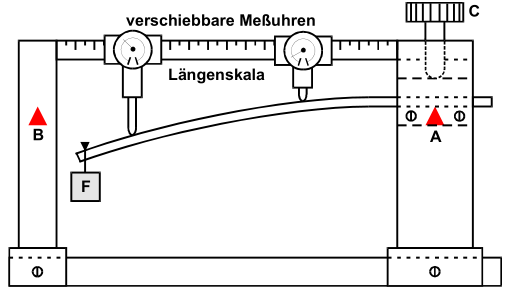
\includegraphics{Messaufbau.PNG}
	\caption{Messapparatur zur Vermessung der Stäbe \cite{sample}}
	\label{fig:messaufbau}
\end{figure}
Als erste Messreihe wurde die Messung der beidseitigen Einspannung durchgeführt. Dafür wurde der betrachtete Stab mit der Länge 57 cm an beiden Seiten der Messapparatur gelagert und es wurde ein Gewicht von 949,9 g (einzelnd abgewogen) an der Mitte des Stabes befestigt. Dann wurde die, durch die Belastung hervorgerufene, Auslenkung des Metallstabs an verschiedenen Messpositionen mit den beiden Messuhren gemessen. Für jeden Messpunkt wurde die Position der Messuhr und die gemessene Verbiegung des Stabs notiert. Dabei wurden mit beiden Messuhren jeweils sechs Werte aufgenommen, sodass insgesamt zwölf Messpunkte ermittelt wurden. \newline
Anschließend wurden die Messungen für die einseitige Einspannung vorgenommen. Dafür wurden beide Stäbe jeweils gemäß Abbildung \ref{fig:messaufbau} eingespannt und an ihrem Ende mit einem Gewicht von 949,9 g (einzelnd abgewogen) belastet. Bei der Wahl des Gewichts wurde darauf geachtet, dass die maximalen Durchbiegungen ungefähr zwischen 3 und 7 mm liegen. Auch hier wurden dann die Verbiegungen der Stäbe an verschiedenen Messpositionen gemessen. Für die einseitige Einspannung wurden für beide Stäbe und für beide Messuhren jeweils zehn Werte gemessen, sodass pro Stab 20 Messpunkte notiert wurden.  
Bei allen Messungen wurde darauf geachtet, dass die Messuhren vor dem Anhängen des Gewichts genullt sind, da auch ein unbelasteter Stab eine leichte Durchbiegung aufweist und die Messuhren bereits durch leichtes Wackeln am Tisch Veränderungen zeigten.